\section{Theorie}
\label{sec:Theorie}
Ziel des Versuches ist die Funktionsweise des Lock-In-Verstärkers kennen zu lernen.
Ein Lock-In-Verstärker entrauscht und verstärkt ein verrauschtes Eingangssignal.\\
Das eingehende Meßsignal wird mit einer Referenzfrequenz $\omega_0$ moduliert.
In Abbildung \ref{fig:aug} wird der grundsätzliche Aufbau des Verstärkers dargestellt.
\begin{figure}
    \centering
    \caption{Schematischer Aufbau des Lock-In-Verstärkers.\cite{v303}}
    \label{fig:aug}
    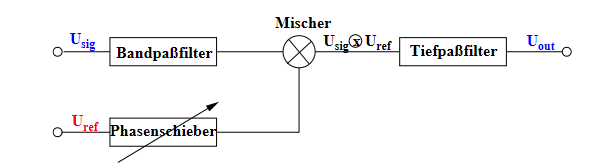
\includegraphics[width = 0.6 \textwidth]{pics/gauf.png}
\end{figure}
Das verrauschte Signal wird durch einen Bandpass von Rauschanteilen höherer und tieferer Frequenzen befreit. In einem Mischer
wird mit einem Referenzsignal der Frequenz $\omega_0$ das Signal multipliziert. Mit Hilfe eines Phasenverschiebers kann die Phasenlage $\varphi$
des Referenzsignals variiert werden und so mit dem Signal synchronisiert werden. Hinter dem Mischer ist ein Tiefpass eingeschaltet, der das Mischsignal $U_\text{sig} \times
U_\text{ref}$ über mehrere Perioden der Modulationsfrequenz integriert. Das Ausgangssignal $U_\text{out}$ ist eine Gleichspannung
$U_\text{out} \propto U_0 \cos \varphi $ die proportional zur Eingangsspannung ist.

